\documentclass{webofc}
\usepackage[utf8]{inputenc}
\usepackage{graphicx}
\usepackage[varg]{txfonts}
\usepackage{subcaption}
\usepackage{appendix}
\usepackage{cleveref}
\usepackage{amsmath}
\usepackage{amssymb}
\usepackage{float}
\usepackage{bm}
\usepackage{xcolor}

% \newcommand{\onedot}{\futurelet\@let@token\@onedot}

\newcommand{\onedot}{.\\}

\newcommand{\eg}{\emph{e.g}\onedot} \newcommand{\Eg}{\emph{E.g}\onedot}
\newcommand{\ie}{\emph{i.e}\onedot} \newcommand{\Ie}{\emph{I.e}\onedot}
\newcommand{\cf}{\emph{c.f}\onedot} \newcommand{\Cf}{\emph{C.f}\onedot}
\newcommand{\etc}{\emph{etc}\onedot} \newcommand{\vs}{\emph{vs}\onedot}
\newcommand{\wrt}{w.r.t\onedot} \def\dof{d.o.f\onedot}
\newcommand{\etal}{\emph{et al}\onedot}


\newcommand{\vx}{\ensuremath{\mathbf{x}}}
\newcommand{\vz}{\ensuremath{\mathbf{z}}}
\newcommand{\vy}{\ensuremath{\mathbf{y}}}

\newcommand{\f}{f}

\newcommand{\dsep}{\ensuremath{\;\|\;}}

\newcommand{\pdata}{\ensuremath{p_{\text{data}}}}
% \newcommand{\pfake}{\ensuremath{p_{\text{fake}}}}
\newcommand{\pfake}{\ensuremath{ p_{G} }}

\newcommand{\todo}[1]{{\color{blue}TODO: #1}}

\newcommand{\E}{\ensuremath{\mathbb{E}}}

\newcommand{\geant}{\texttt{Geant4} }


\begin{document}

\title{Generative Models for Fast Calorimeter Simulation}
\subtitle{LHCb case}

\author{
 \firstname{Viktoria} \lastname{Chekalina} \inst{1,2}
\and
    \firstname{Elena} \lastname{Orlova} \inst{3}\fnsep\thanks{\email{egorlova68@gmail.com}}
\and
    \firstname{Fedor} \lastname{Ratnikov} \inst{1,2}
\and
     \firstname{Dmitry} \lastname{Ulyanov} \inst{3}
\and
     \firstname{Andrey} \lastname{Ustyuzhanin} \inst{1,2}
\and
     \firstname{Egor} \lastname{Zakharov} \inst{3}\fnsep\thanks{\email{eo.zakharov@gmail.com}}
}

\institute{
NRU Higher School of Economics, Moscow, Russia
\and
Yandex School of Data Analysis, Moscow, Russia  
\and
Skolkovo Institute of Science and Technology, Moscow, Russia
}
        
\abstract{Simulation is one of the key components in high energy physics. Historically it relies on the Monte Carlo methods which require a tremendous amount of computation resources. These methods may have difficulties with the expected High Luminosity Large Hadron Collider (HL LHC) need, so the experiment is in urgent need of new fast simulation techniques. We introduce a new Deep Learning framework based on Generative Adversarial Networks which can be faster than traditional simulation methods by 5 order of magnitude with reasonable simulation accuracy. This approach will allow physicists to produce a big enough amount of simulated data needed by the next HL LHC experiments using limited computing resources.}


\maketitle


\section{Introduction}

Simulation plays an important role in particle and nuclear physics. It is widely used in detector design and in comparisons between experimental data and theoretical models. Traditionally, simulation relies on \textit{Monte Carlo methods} and requires significant computational resources. In particular, such methods do not scale to meet the growing demands resulting from large quantities of data expected during High Luminosity Large Hadron Collider (HL-LHC) runs. The detailed simulation of particle collisions and interactions as captured by detectors at the LHC using a well-known simulation software \geant annually requires billions of CPU hours constituting more than half of the LHC experiments' computing resources~\cite{bozzi2014,flynn2015computing}. More specifically, the detailed simulation of particle showers in calorimeters is the most computationally demanding step.
 
A line of simulation methods that exploit the idea of reusing previously calculated or measured physical quantities have been developed to reduce the computation time~\cite{grindhammer2000parameterized,atlas2010simulation}. These approaches suffer from being specific to an individual experiment and, despite being faster than the full simulation, they are not fast enough or lack accuracy. Thus, the particle physics community is in need of new faster simulation methods to model experiments. 
    
One of the possible approaches to simulate the calorimeter response is using \textit{deep learning} techniques. In particular, a recent work~\cite{paganini2017calogan}, provided evidence that \textit{Generative Adversarial Networks} can be used to efficiently simulate particle showers. While over $100,000 \times$ speed-up over \geant is achieved, the setup was quite simple as the input particles were parametrized by energy only. However,  even in this simplified approach, there are significant differences in distributions between generated and original parameters. 

In this work we build a model upon \text{Wasserstein Generative Adversarial Networks} and show its superior performance over approach~\cite{paganini2017calogan}. We also evaluate our model in a more complex scenario, when a particle is described by $5$ parameters: 3d momentum $(p_x,~ p_y,~ p_z)$ and 2d coordinate $(x,~ y)$. Our method for high-fidelity fast simulation of particle showers in the specific LHCb calorimeter aims to replace the existing Monte Carlo based methods and achieve a significant speed-up factor.
 





\section{Related work}
Generative models are of great interest in deep learning. With these models one can approximate a very complex distribution defined by a set of its samples. 
For example, such models can be utilized to generate a face image of a never existed person or to continue a video sequence given several initial frames. 
In this section we give a brief overview of the most popular generative model in computer vision — Generative Adversarial Networks (GANs),
 its strong and weak sides and different modifications to alleviate its weaknesses. Then we review and analyse current approaches for applying GANs to 
the simulation of calorimeters in High energy physics.


\subsection{From GANs to WGANs}

Genarative Adversarial Networks (GANs) were originally presented by I.~Goodfellow~\etal in 2014 \cite{goodfellow2014generative} and quickly became a state-of-the-art technique in areas such as image generation \cite{radford2015unsupervised} with huge number of extensions \todo{\cite{1,2,3,4}}.


In the GAN framework the aim is to learn a \textit{generator} $G$ to warp an easy-to-draw distribution $p(\vz)$ (e.g. $p(\vz) = \mathcal{N}(0, I)$ ) into a target distribution $\pdata(\vx)$. In this case the sampling from target distribution $\pdata(\vx)$ is done by first drawing a sample from the distribution $p(\vz)$ and then feeding it into the generator: $G(\vz) \sim \pdata(\vx)$, where $\vz \sim p(\vz)$. For such sampling procedure, the time needed to draw a sample from $\pdata(\vx)$ is approximately equal to the time needed to evaluate the function $G$ in a point.  

The generator is learned by using a feedback from an external classifier (usually called \textit{discriminator}), which tries to find discrepancy between the target distribution $\pdata(\vx)$ and fake distribution defined by samples from the generator $G(\vz),\, \vz \sim p(\vz)$. The process in summarized in~\cref{fig:GANs}.

\begin{figure}
\centering
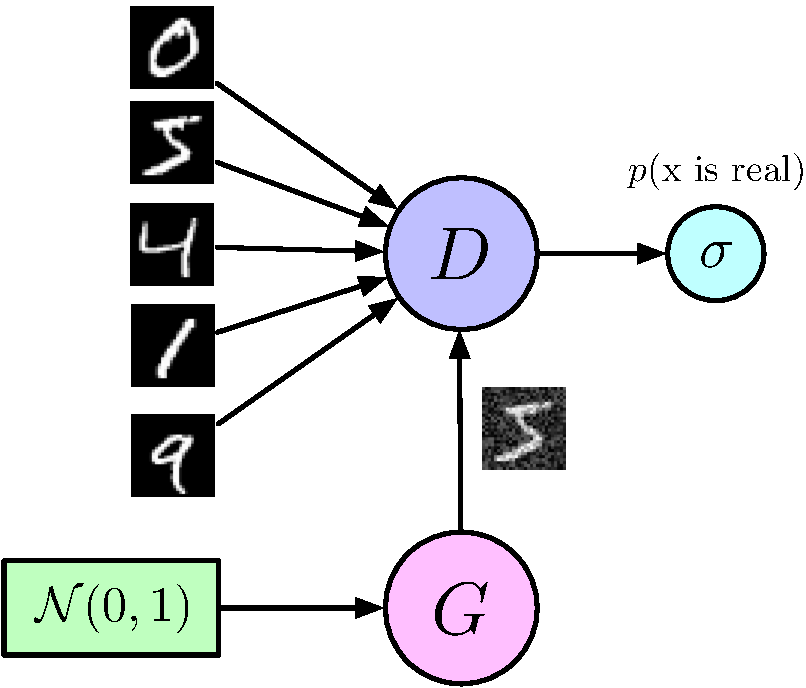
\includegraphics[width=0.3\linewidth]{figures/gan_pic.pdf}
\caption{Generative Adversarial Networks for digit generation. The generator $G$ transforms the noise vector $\vz \sim p(z)$ to an image of a digit and the discriminator $D$ classifies inputs as real digits or fake digits from generator. Generator and discriminator are trained in an adversarial manner: the task of $G$ is to make it imporssible for $D$ to distinguish between the real and fake digits as in this case $G$ reproduces the data distribution $\pdata$.}\label{fig:GANs}
\end{figure}


More formally, generator $G$ and discriminator $D$  ... game : 
\begin{equation}\label{eq:gan}
\min_G \max_D \E_{\vx \sim \pdata(\vx)} [\log D(\vx)] + \E_{\vz \sim p(\vz)} [\log(1 - D(G(\vz)))],
\end{equation} 
where $\vx \sim \pdata(\vx)$ are samples from the input data, $\vz \sim p(\vz)$ are the random noise samples, $G(\vz)$ are the generated images and $D(G(\vz))$ is the output of the discriminator specifying the probability of its input to belong to class <<real>>.

In practice this ojective is optimized using alternating gradient descent. For a fixed generator, the discriminator minimizes binary cross-entropy in a binary classification problem (samples from target distribution versus samples from generator a.k.a. fake distribution). For a fixed discriminator, generator is updated to make its samples to be misclassified by discriminator, thus moving fake distribution closer to the target.   

It is possible to show, that for a fixed generator the solution for the inner optimization can be written analitically: 
\begin{equation}\label{eq:gan}
\max_D \E_{\vx \sim \pdata(\vx)} [\log D(\vx)] + \E_{\vz \sim p(\vz)} [\log(1 - D(G(\vz)))] = \text{JS}( \pdata(\vx) \| \pfake(\vx))
\end{equation} 
where $JS$ is Jenson-Shennon divergence. 

The interpretation is the following: for the fixed generator, the discriminator computes the divergence between the target and fake distributions, while the generator aims to update fake distribution to make this divergence lower:

\begin{equation}\label{eq:ganJS}
\min_G \text{JS}( \pdata(\vx) \| \pfake(\vx))
\end{equation} 

While Jenson-Shennon divergence arises from the original \label{eq:gan}, any divergence or distance can be used instead.

I recent work~\cite{arjovsky2017wasserstein} proposed to use \textit{Wasserstein distance} and proved ... 

\begin{equation}\label{eq:wasserstein_metric}
W(\pdata(\vx) \| \pfake(\vx) ) = \max_{f \in \mathbb{F}} \E_{\vx \sim \pdata(\vx)}[f(\vx)] - \E_{\vx \sim \pfake} [f(\vx)]
\end{equation}
where $\mathbb{F}$ is a set of 1-Lipshitz functions.

which leadas to the following game: 


\begin{equation}\label{eq:wasserstein_metric}
\min_G \max_{f \in \mathbb{F}} \E_{\vx \sim \pdata(\vx)}[f(\vx)] - \E_{\vz \sim p(\vz)} [f(G(\vz))]
\end{equation}

% When parametri
\begin{equation} \label{gpwgan-loss}
\begin{gathered}
\mathcal{L}(\bm{\theta}) =
\underbrace{ \underset{\tilde{\vx} \sim \mathbb{P}_g}{\mathbb{E}}  \Big[D(\tilde{\vx})\Big] - \underset{\vx \sim \mathbb{P}_r}{\mathbb{E}} \Big[D(\vx)\Big]}_{\text{original loss}} + 
\underbrace{ \lambda \underset{\vx \sim \mathbb{P}_g}{\mathbb{E}} \Big[\big(\|\nabla_{\tilde{\vx}} D(\tilde{\vx})\|_2 - 1\big)^2 \Big]}_{\text{gradient penalty}}.
\end{gathered}
\end{equation}




% \subsubsection{Wasserstein GAN}
% There are various modifications of GANs for struggling with some typical problems and for improving the training procedure. A common GANs issue is so--called mode collapse when $p_\text{model} (\vx)$ fails to capture a multimodal nature of $\pdata(\vx)$ and in extreme cases all the generated samples might be identical, in more involved architectures such as Waserstain GAN \cite{arjovsky2017wasserstein} the discriminator loss is argued to be consistent with the image quality. The main idea is to apply the Wasserstein-1 distance in order to compare $\pdata$ and $p_{\text{model}}$.

% Let $\mathbb{X}$ be a compact metric set and let $\mathbb{B}$ denote the set of all the Borel subsets of $\mathbb{X}$. Let $Prob(\mathbb{X})$ denote the space of probability measures defined on $\mathbb{X}$. The \emph{Earth-Mover} or \emph{Wasserstein-1} distance between two distributions $\mathbb{P}_r, \mathbb{P}_g \in Prob(\mathbb{X})$ is defined in the following way:

% \begin{equation}\label{wasserstein_metric}
% W(\mathbb{P}_r, \mathbb{P}_g) = \inf_{\gamma \in \Pi(\mathbb{P}_r, \mathbb{P}_g)} \mathbb{E}_{(x, y) \sim \gamma} \big{[}\|\vx-\textbf{y}\|\big{]},
% \end{equation}

% where $\Pi(\mathbb{P}_r, \mathbb{P}_g)$ is the set of all joint distributions $\gamma(x, y)$ whose marginals are respectively $\mathbb{P}_r$ and $\mathbb{P}_g$. $\gamma(x, y)$ denotes how much “mass” must be transported from $x$ to $y$ in order to transform the distributions $\mathbb{P}_r$ into the distribution $\mathbb{P}_g$. Thus, the Wasserstein distance can be defined as the minimum cost of transporting mass in order to transform the distribution $\mathbb{P}_r$ into the distribution $\mathbb{P}_q$. 

% By applying to this distance the \emph{Kullback--Leibler divergence}, the \emph{Jensen-Shannon divergence} and the Kantorovich--Rubinstein duality and also parameterization of family of functions $\{f_w\}_{w \in \mathcal{W}}$ that are all K-Lipschitz for some K we could consider solving the problem (for more detailed information see the paper \cite{arjovsky2017wasserstein})

% \begin{equation}\label{optim}
% \max_{w \in \mathcal{W}} \mathbb{E}_{x \sim P_r}[f_w(x)] - \mathbb{E}_{z\sim p(z)} [f_w(g_\theta(z))]
% \end{equation}

% and if the supremum in \eqref{optim} is attained for some $w \in \mathcal{W}$, this process would lead to a calculation of $W(\mathbb{P}_r, \mathbb{P}_\theta)$ up to a multiplicative constant.
% So, the WGAN value function is
% \begin{equation}\label{wgan_loss}
% \min_G \max_{D \in \mathcal{D}}  \mathbb{E}_{\vx \sim \mathbb{P}_r}  [D(\vx)] - \mathbb{E}_{\tilde{\vx} \sim \mathbb{P}_g} [D(\tilde{\vx})],
% \end{equation}
% where $\mathcal{D}$ is the set of 1-Lipschitz functions and $\mathbb{P}_g$ is  the model distribution defined by $\tilde{\vx} = G(\vz), ~\vz \sim p(\vz).$

% In general, the training procedure of GANs is known to be difficult and presents such issues as mode collapse, and WGAN often helps to overcome this problem.

% The Wasserstein GAN value function makes optimization process easier because the discriminator's gradient with respect to its input is better behaved than its GAN counterpart. Also, it was noticed that the WGAN value function tend to correlate with the original data quality which is not always the case for ordinary GANs.


\subsubsection{Wasserstain GAN with gradient penalty}
An alternative way to enforce the Lipschitz constraint was introduced in \cite{gulrajani2017improved}. The authors consider directly constraining the gradient norm of the discriminator's output with respect to its input because a differentiable function is 1-Lipschtiz if and only if it has gradients with norm at most 1 everywhere. To come over tractability issues a soft version of the constraint with a penalty on the gradient norm for random samples $\tilde{\vx} \sim \mathbb{P}_{\tilde{\vx}}$ was suggested. Therefore, a new obtained objective is 
\begin{equation} \label{gpwgan-loss}
\begin{gathered}
\mathcal{L}(\bm{\theta}) =
\underbrace{ \underset{\tilde{\vx} \sim \mathbb{P}_g}{\mathbb{E}}  \Big[D(\tilde{\vx})\Big] - \underset{\vx \sim \mathbb{P}_r}{\mathbb{E}} \Big[D(\vx)\Big]}_{\text{original loss}} + 
\underbrace{ \lambda \underset{\vx \sim \mathbb{P}_g}{\mathbb{E}} \Big[\big(\|\nabla_{\tilde{\vx}} D(\tilde{\vx})\|_2 - 1\big)^2 \Big]}_{\text{gradient penalty}}.
\end{gathered}
\end{equation}

This approach demonstrates strong modeling performance and stability across a variety of architectures.  Now it is a state-of-the-art technique in GANs. 
How to calculate this loss in practice is described on~\cref{sec:training_strategy}.

\subsection{GANs in high energy physics}
The first \todo{strong claim! is it 100\% true? what about LAGAN https://arxiv.org/pdf/1701.05927.pdf?} systematic study on the application of deep learning to particle physics has been carried out by Paganini et al. in 2017 \cite{paganini2017calogan} and called CaloGAN. The authors aim to speedup particle simulation in a 3-layer unheterogeneous calorimeter at the LHC using GANs framework and achieve $\sim 10^5 \times$ speedup. They use an existing state-of-the-art (but slow) simulation engine \geant to create a training dataset. They simulated positrons, photons and charged pions with various energies from 1 GeV to 100 GeV \todo{with energies are incident perpendicular on the center of the calorimeter front}. The shower in the first layer is represented as a $3 \times 96$ image, the middle layer as a $12 \times 12$ image, and the last layer as a $12 \times 6$ image. 

Their desing of the generator network is based on DCGAN structure \cite{radford2015unsupervised} with some convolutional layes replaced by locally-connected layers \cite{taigman2014deepface}. The idea of locally connected layers is based on the fact that every pixel position gets its own filter while an ordinary convolutional layer is applied over the whole image, independently of location. Spreading of this method to particle physiscs simulation has been described in the previous work of the authors and such type of neural network was called LAGAN \cite{de2017learning}. A special section in the paper is devoted to the evaluation of the quality of the CaloGAN produced images where  sparsity level,  energy per layer or total energy are suggested to measure the performance of the model. 

The obtained results demonstrate a prospect of application of GANs for the particle showers generation and replacing of the Monte Carlo methods with the proposed approach. The CaloGAN shows sizable simulation-time speed ups compared to \geant. 

In fact, the CaloGan model is based on DCGAN with the described tricks. However, GANs tend to suffer from mode collapse. Therefore, the CaloGan architecture cannot be applied for all datasets, because there is a high probability of mode collapse appearance and it is a limitation of this work.

\section{Dataset}
In this work we focused on electrons interactions inside the electromagnetic calorimeter inspired by the LHCb detector on the LHC at CERN \cite{Alves:2008zz} . The calorimeter used in this study uses "shashlik" technology of alternating scintillating tiles and lead plates. The prototype  consists of 5 $\times$ 5 blocks of size 12 cm $\times$ 12 cm, the cell granularity corresponds to each block is 6 $\times$ 6 of size 2 cm $\times$ 2 cm. There are 66 total layers in ECAL, 2 mm lead absorber and 4 mm scintillator each. In fact, the shower appears in 3d, but all energies deposited in all scintillator layers of one cell are summed up. This procedure reproduced the actual shower energy collection in the calorimeter. Thus, the calorimeter response can be represented as 30 $\times$ 30 images $Y$ with the corresponding parameters $(p_x,~ p_y,~ p_z,~ x,~ y)$ of the original particle. Such image example is presented in~\cref{fig:real-imgs}.

The training data set is created as follows. The calorimeter prototype structure described above is described in \geant as a corresponding mixture of sensitive and insensitive volumes. Particles are generated using Particle Gun. Particle energies are distributed as $1/E$ in energy range between 1 and 100 GeV. Particle positions are generated uniformly in the square 1$\times$1 cm in the center of the calorimeter face. Finally, particle angles are distributed normally with widths of 20 degree in $XZ$ plane and 10 degree in $YZ$ plane. Then \geant  is used to simulate particle interaction with the calorimeter using the full set of corresponding physics processes. Information about every event therefore includes the original particle parameters accompanied by 30 $\times$ 30 matrix of energies deposited in scintillator for every cell tower $Y$. Electrons are used as a test particles. Produced raining dataset contains 50 000 events, and another 10 000 events are used as a  test data sample.

\section{Our model} \label{sec:model}
Our idea is to treat simulations as a black-box and replace the traditional Monte Carlo simulation with a method based on Generative Adversarial Networks. WGANs with gradient penalty are considered to be state-of-the-art technique for image producing, so we decide to implement a tool based on this particular approach. For it to be useful in realistic physics applications such a system needs to be able to accept requests for the generation of showers originating from an incoming particle parameters such as 3d momentum and 2d coordinate. We introduce an auxiliary task of energy reconstruction to condition on these parameters $p_x$, $p_y$, $p_z$ and $x$, $y$.

\subsection{Model architecture}



We need to generate a specific calorimeter response to a particle with some parameters. It means that a model is required to be conditional.
% sampling not just from $p(\textbf{y}),$ but from $p(\textbf{y}|\vx),$ so, 
Firstly, we describe a generator and discriminator architecture. The generator maps from an input (a 512 $\times$ 1 vector sampled from the Gaussian distribution and the particle parameters) to an 30 $\times$ 30 image $\hat{\textbf{y}}$ using deconvolutional layers (in fact, it is an upsampling procedure and convolutions) which are arranged as follows. We concatenate the noise vector and the parameters $(p_x,~ p_y,~ p_z,~ x,~ y)$, after that we add a fully connected layer with reshaping and obtain 256 $\times$ 4 $\times$ 4 output. After a sequence of 2d deconvolutions we get outputs of size  128 $\times$ 8 $\times$ 8, 64 $\times$ 15 $\times$ 16 and 32 $\times$ 32 $\times$ 32  with ReLu activation functions. After this procedure we crop the last output to obtain the image of desired size 30 $\times$ 30.

As for the discriminator, it takes a batch of images as input (all images in the batch are real or generated by $G$) and returns the score $D(\textbf{y})$ or $D(\hat{\textbf{y}})$ as it is described in \cite{arjovsky2017wasserstein}. Discriminator architecture is simply the reversed generator architecture (i.e. sizes of layers go in the opposite order). It implies that we have 30 $\times$ 30 matrix as input, then we obtain layers outputs of size 32 $\times$ 32 $\times$ 32, 64 $\times$ 15 $\times$ 16, 128 $\times$ 8 $\times$  8, after that reshaping leads to 256 $\times$ 4 $\times$ 4, and by applying LeakyRelu activation function we get the final score. The model scheme is presented in~\cref{fig:model}.

\begin{figure}
\centering
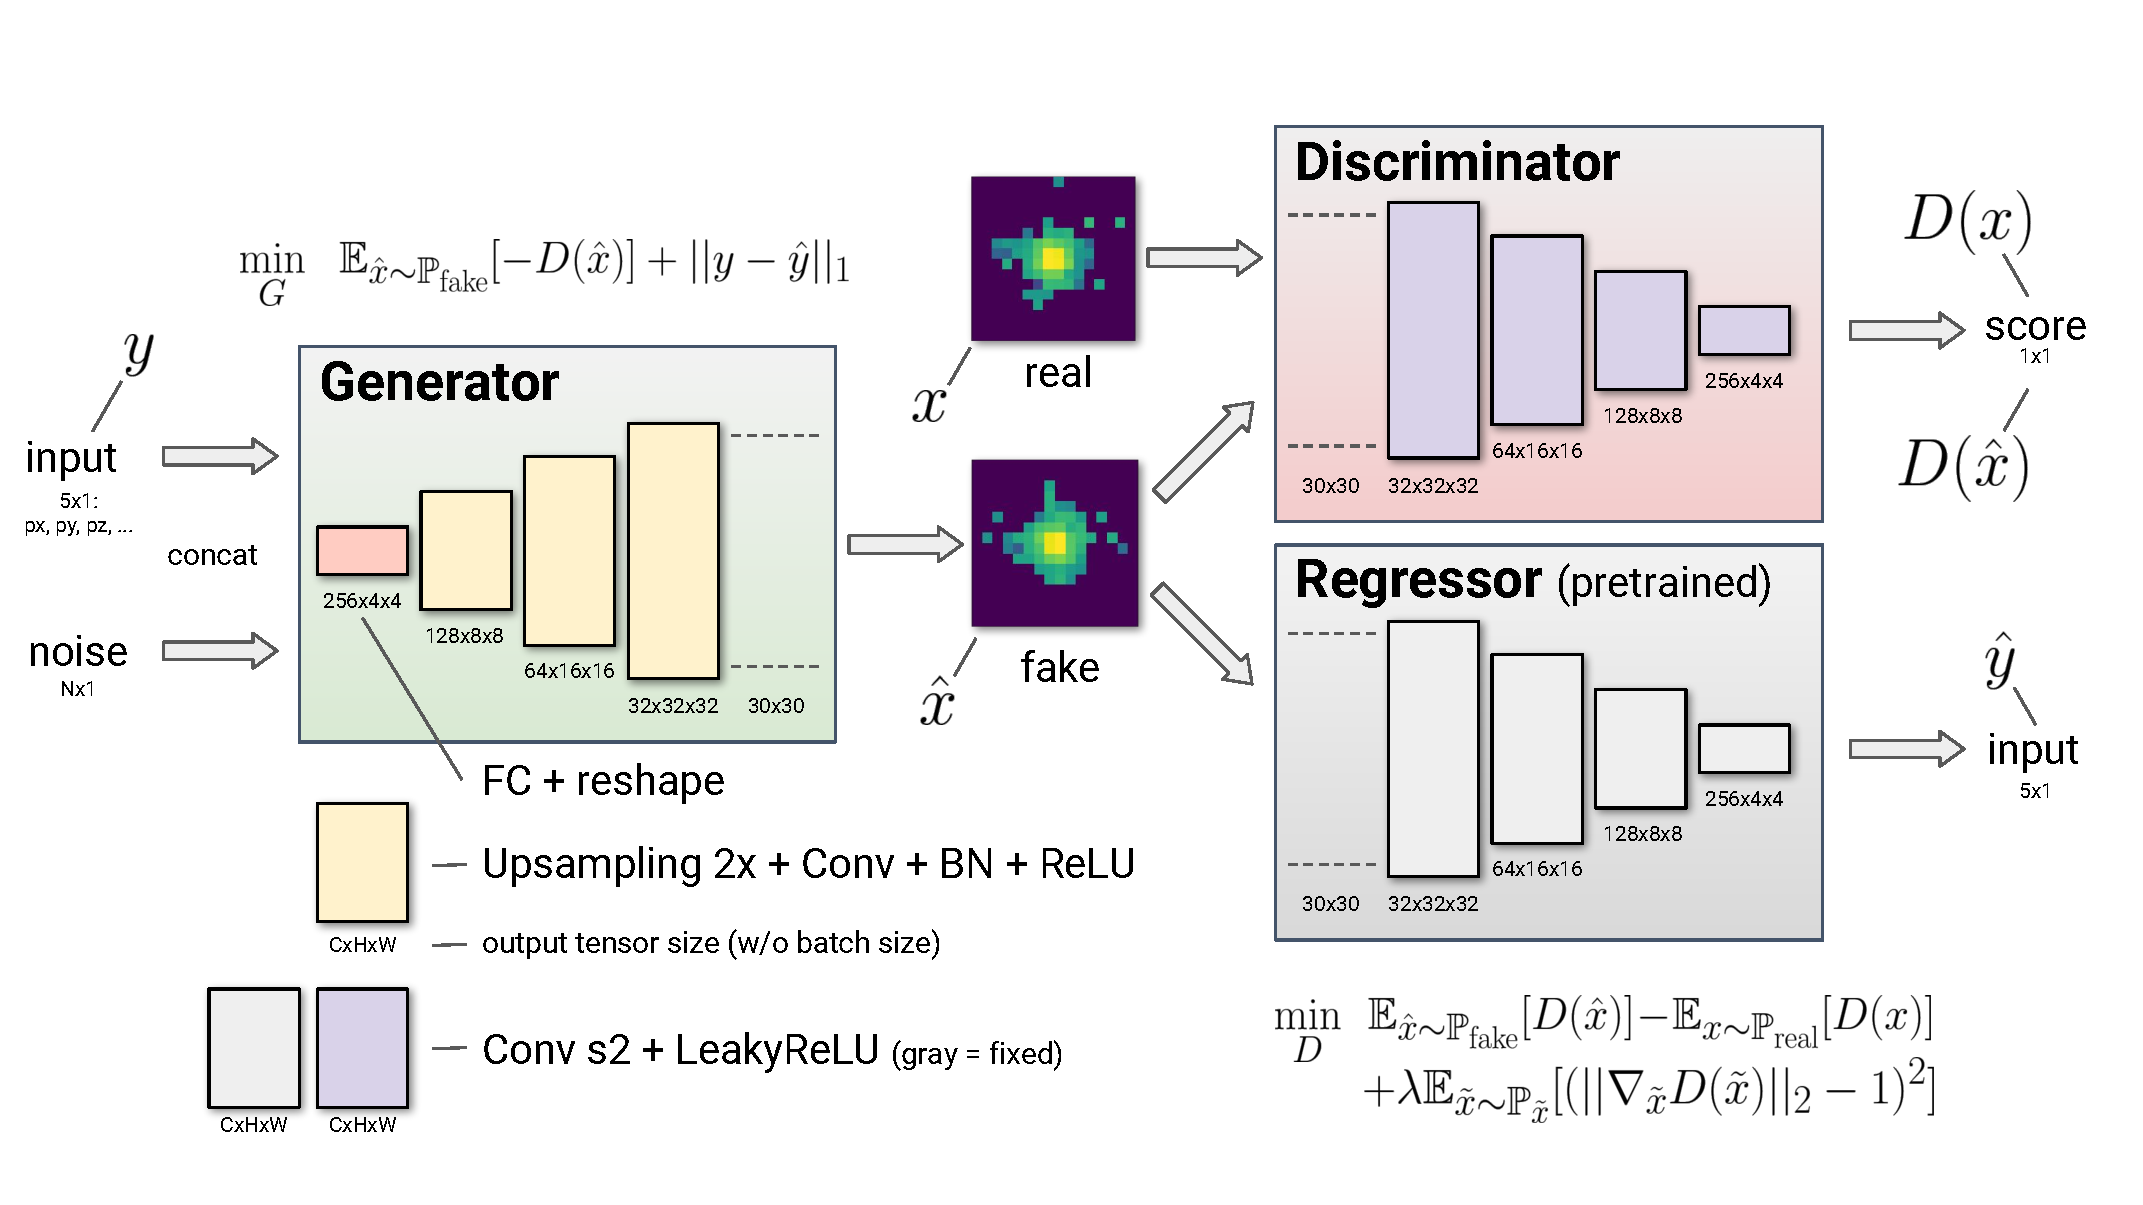
\includegraphics[width=1\textwidth]{figures/model_architecture.pdf}
\caption{Model architecture. Pre-trained regressor for the particle parameters prediction makes our model conditional. Thanks to building up the information from the pre-trained regressor into the discriminator gradient we learn $G$ to produce a specific calorimeter response.}\label{fig:model}
\end{figure}

How to train WGAN with gradient penalty in conditional manner is described in the following section.

\subsection{Training strategy} \label{sec:training_strategy}
Due to the nature of WGAN loss, conditioning on the continuous value is a non-trivial task. To overcome this issue we suggest to embed a pre-trained regressor in our model. We train a neural network to predict the particle parameters by the calorimeter response. As for architecture, it has the same one as the discriminator but with a perceptual loss described in \cite{johnson2016perceptual} because, as we figured out, it works better rather than standard MSE. By building up the information from the pre-trained regressor into the discriminator gradient, we obtain the conditional model because we train the generator and the discriminator together. Now the discriminator makes the generator produce a specific calorimeter response.

Matrices from our dataset are pretty sparse because almost all information is located in central cells (see~\cref{fig:real-imgs}). To make optimization process easier we apply a box--cox transformation. This mapping helps to smooth the data that makes the optimization process more stable.
Results obtained with the described model are presented in the following section.

\begin{figure}
\begin{center}
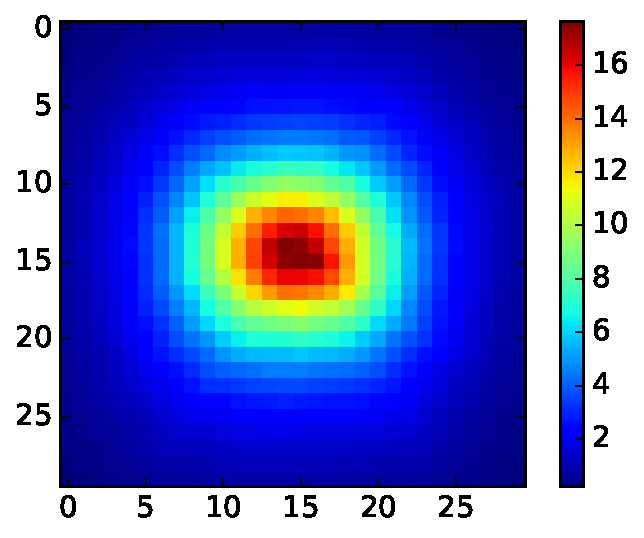
\includegraphics[width=0.5\textwidth]{figures/mean_cluster.pdf}
\caption{energy deposition in different cells of used 30$\times $30 setup for \geant simulated events averaged over all events in the used dataset. \label{fig:real-imgs}}
\end{center}
\end{figure}
\section{Experiments}

\begin{figure}
\captionsetup[subfigure]{justification=centering}
  \centering
  \begin{subfigure}{0.24\textwidth}
    \centering
    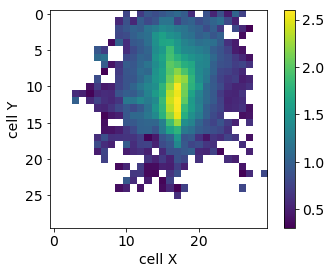
\includegraphics[width=1\textwidth]{figures/1_real.png}
    % \caption{\\$E = 63.7~\text{GeV}$ \\ $\frac{p_x}{p_z}=0.005$ \\ $\frac{p_y}{p_z}=0.154$}\label{fig:real-imgs-1}
  \end{subfigure}
  \begin{subfigure}{0.24\textwidth}
    \centering
    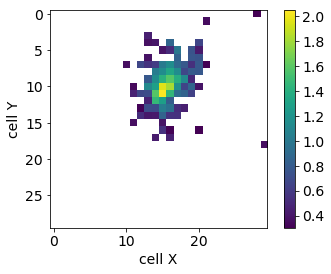
\includegraphics[width=1\textwidth]{figures/2_real.png}
    % \caption{\\$E = 6.5~\text{GeV}$ \\  $\frac{p_x}{p_z}=0.0046$ \\$\frac{p_y}{p_z}=0.108$}\label{fig:real-imgs-2}
  \end{subfigure}
    \begin{subfigure}{0.24\textwidth}
    \centering
    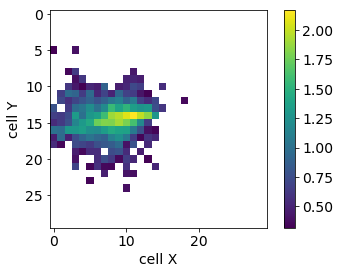
\includegraphics[width=1\textwidth]{figures/3_real.png}
    % \caption{\\$E = 15.6~\text{GeV}$ \\ $\frac{p_x}{p_z}=0.196$ \\ $\frac{p_y}{p_z}=-0.036$}\label{fig:real-imgs-3}
  \end{subfigure}
  \begin{subfigure}{0.24\textwidth}
    \centering
    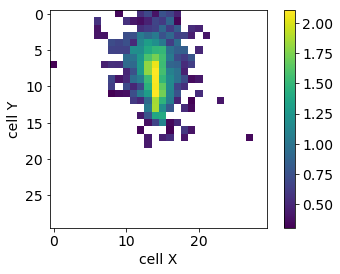
\includegraphics[width=1\textwidth]{figures/4_real.png}
    % \caption{\\$E = 15.6~\text{GeV}$ \\  $\frac{p_x}{p_z}=-0.019$ \\ $\frac{p_y}{p_z}=0.181$}\label{fig:real-imgs-4}
  \end{subfigure}\\
   \begin{subfigure}{0.24\textwidth}
    \centering
    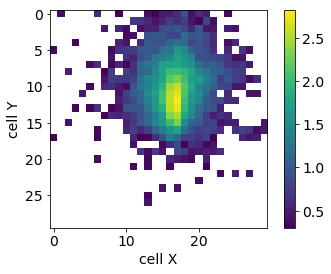
\includegraphics[width=1\textwidth]{figures/1_gen.png}
    \caption{\\$E_0 = 63.7~\text{GeV}$ }%\\ $\frac{p_x}{p_z}=0.005$ ,  $\frac{p_y}{p_z}=0.154$}}%\label{fig:gen-imgs-1}
  \end{subfigure}
  \begin{subfigure}{0.24\textwidth}
    \centering
    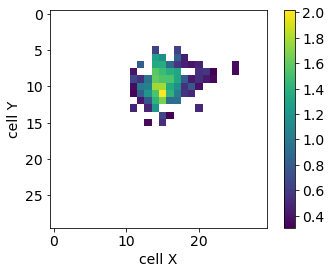
\includegraphics[width=1\textwidth]{figures/2_gen.png}
    \caption{\\$E_0 = 6.5~\text{GeV}$ }% \\  $\frac{p_x}{p_z}=0.046$ , $\frac{p_y}{p_z}=0.108$}}%\label{fig:gen-imgs-2}
  \end{subfigure}
    \begin{subfigure}{0.24\textwidth}
    \centering
    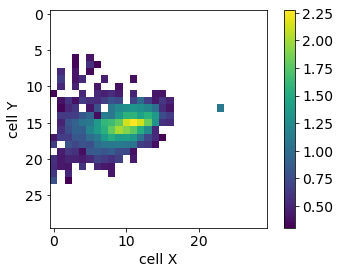
\includegraphics[width=1\textwidth]{figures/3_gen.png}
    \caption{\\$E_0 = 15.6~\text{GeV}$ }% \\ $\frac{p_x}{p_z}=0.196$ ,  $\frac{p_y}{p_z}=-0.036$}}%\label{fig:gen-imgs-3}
  \end{subfigure}
  \begin{subfigure}{0.24\textwidth}
    \centering
    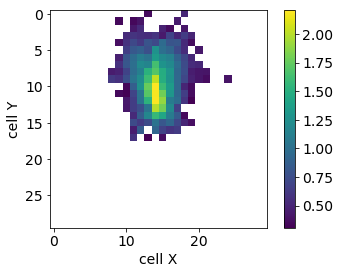
\includegraphics[width=1\textwidth]{figures/4_gen.png}
    \caption{\\$E_0 = 15.9~\text{GeV}$ }% \\  $\frac{p_x}{p_z}=-0.019$ ,  $\frac{p_y}{p_z}=0.181$}}%\label{fig:gen-imgs-4}
  \end{subfigure}
 
  \caption{Showers generated with \geant (first row) and the showers,
    simulated with our model (second row) for three different sets of
    input parameters. Color represents $log_{10}(\frac{E}{MeV})$ for every cell}
  \label{fig:geant_vs_ours}
\end{figure}

We start with comparing original clusters, produced by full \geant
simulation and clusters generated by the trained model for the same
 parameters of the incident particles: the same energy, the same direction,
 and the same position on the calorimeter face. Corresponding images
 for four arbitrary parameter sets are presented
 in~\cref{fig:geant_vs_ours}. These images demonstrate very good
 visual similarity between simulated and generated clusters.


\begin{figure}
  \centering
  \begin{subfigure}[t]{0.3\textwidth}
    \centering
    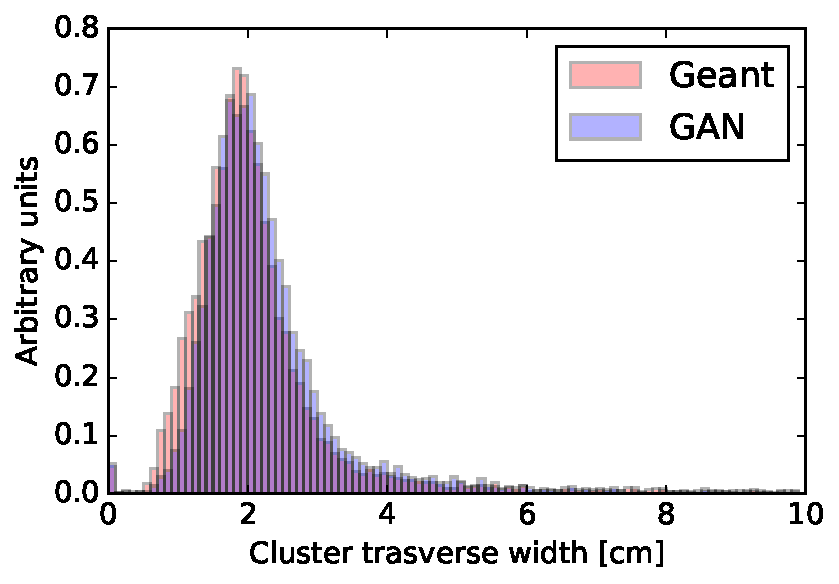
\includegraphics[width=1\textwidth]{figures/width_trans.pdf}
    \caption{The transverse width of real and generated clusters}
  \end{subfigure}\hspace{0.2\textwidth}
 \begin{subfigure}[t]{0.3\textwidth}
    \centering
    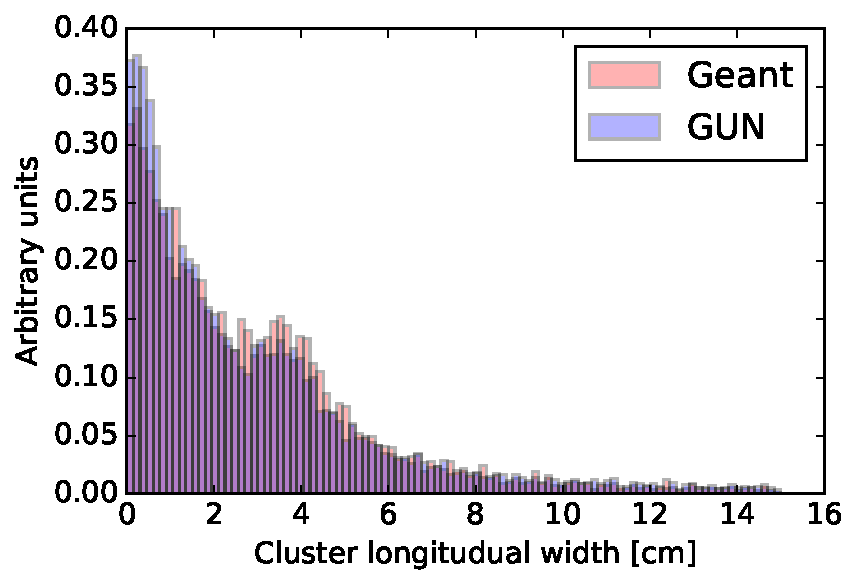
\includegraphics[width=1\textwidth]{figures/width_long.pdf}
    \caption{The longitudinal width of real and generated clusters}
  \end{subfigure}
  \begin{subfigure}[t]{0.3\textwidth}
    \centering
    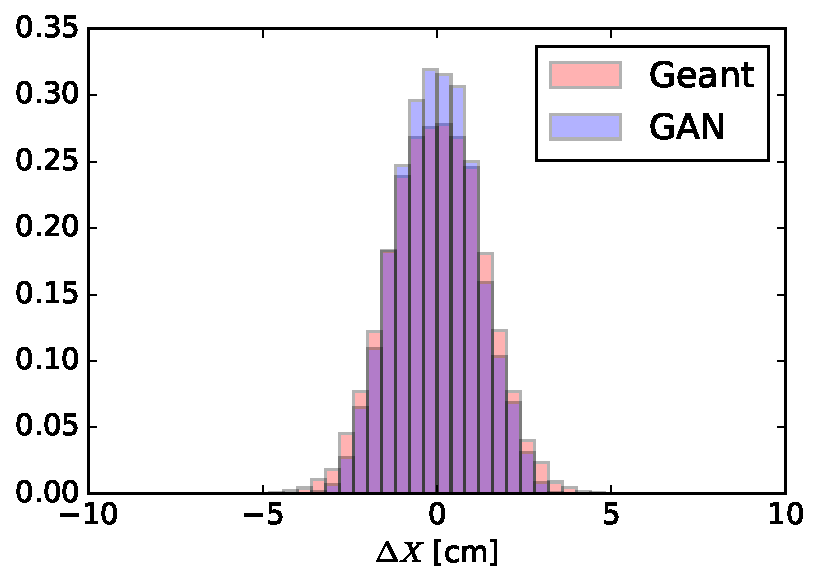
\includegraphics[width=1\textwidth]{figures/deltaX.pdf}
    \caption{$\Delta X$ between cluster center of mass and the true particle coordinate}
  \end{subfigure}\hspace{0.2\textwidth}
  \begin{subfigure}[t]{0.3\textwidth}
    \centering
    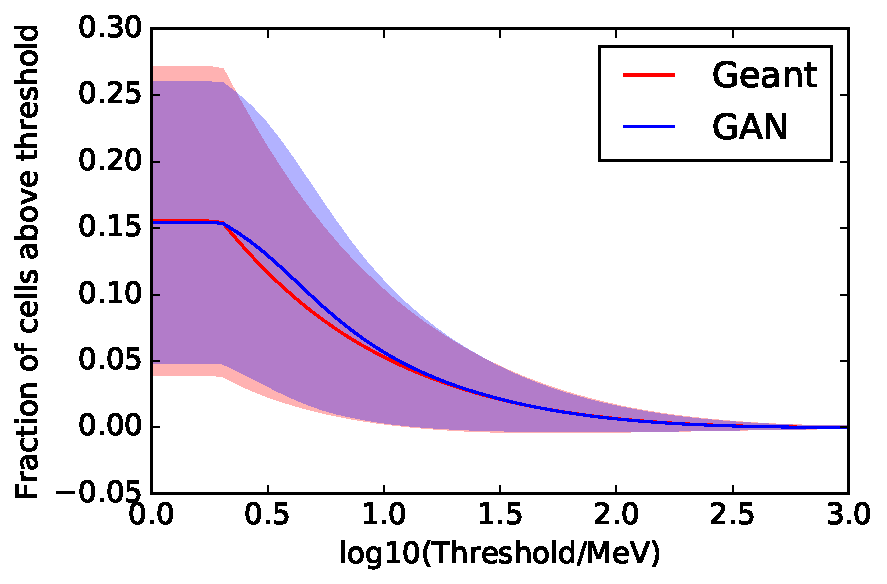
\includegraphics[width=1\textwidth]{figures/sparsity.pdf}
    \caption{The sparsity of real and generated clusters}
  \end{subfigure}
  \begin{subfigure}[t]{0.3\textwidth}
    \centering
    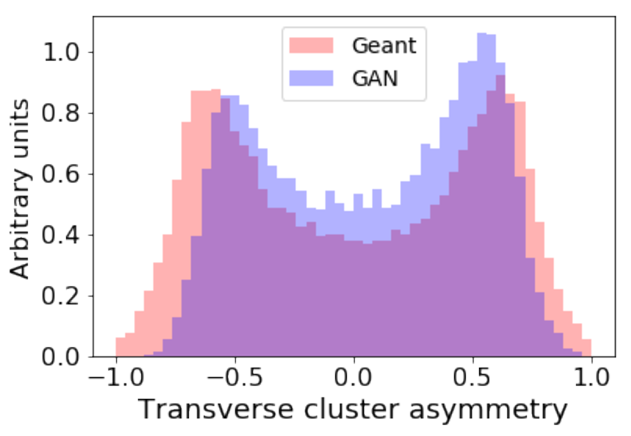
\includegraphics[width=1\textwidth]{figures/transverseAsymmetry.pdf}
    \caption{The transverse asymmetry of real and generated clusters}
  \end{subfigure}\hspace{0.2\textwidth}
  \begin{subfigure}[t]{0.3\textwidth}
    \centering
    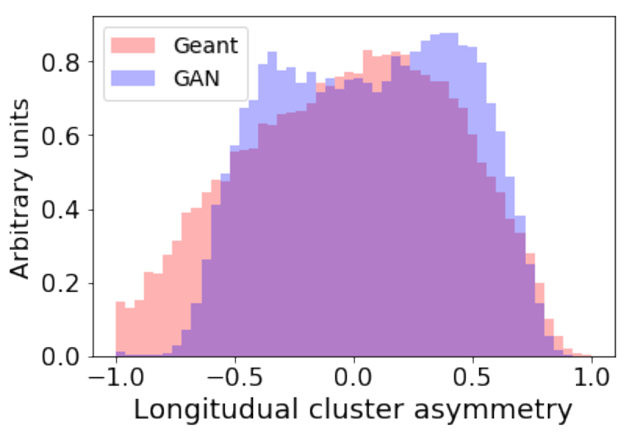
\includegraphics[width=1\textwidth]{figures/longAsymmetry.pdf}
    \caption{The longitudinal asymmetry of real and generated clusters}
  \end{subfigure}
  \caption{Generated images quality evaluation including described physical characteristics.}\label{fig:quality}  
\end{figure}

Then we continue with quantitative evaluation of the proposed simulation
method. While generic evaluation methods for generative models exist,
here we base our evaluation on physics-driven similarity
metrics. These metrics are designed using the domain knowledge and the
recommendations from physicists on the evaluation of simulation
procedures. 
For this presentation we selected few cluster properties which essentially
drive cluster properties used in the reconstruction of calorimeter objects
and following physics analysis. If initial particle direction is not
perpendicular to the calorimeter face, produced cluster is elongated
in that direction. Therefore we consider separately cluster width in
the direction of the initial particle and in the transverse
direction. Spatial resolution, that is the distance between center
mass of the cluster and the initial track projection to the shower max
depth, is another important characteristics affecting physics
properties of the cluster. Cluster sparsity, that is the fraction of
cells with energies above some threshold, reflects marginal low
energy properties of the generated clusters. Finally, longitudinal and
transverse asymmetries, that are differences in energies between
forward-backward and left-right sides of the cluster, characterise
coherent energy variations.  
 These  characteristics are presented in~\cref{fig:quality}. 

The primary cluster characteristics  demonstrate good agreement with
fully simulated data. However secondary characteristics driven by
long range correlations between different cluster contributions might
be significantly improved.  




As for model performance, we trained our model for 3000 epochs which takes about 70 hours on GPU NVIDIA Tesla K80. The sampling rate is 0.07 ms per sample on GPU, 4.9 ms per sample on CPU.

\section{Conclusion and future outlook}\label{conclusion}

The research proves that Generative Adversarial Networks are a good candidate for fast simulating of high granularity detectors typically studied for the next generation accelerators. We have successfully generated images of shower energy deposition with a condition on the particle parameters such as the momentum and the coordinate using modern generative deep neural network techniques such as Wasserstain GAN with gradient penalty.

Future work will be focused improving obtained results such as shower shape characteristics.



\bibliography{caloGAN_chep2018}


%\appendix
%\section{Appendix}
To define cluster parameters let us consider one calorimeter response produced by one particle. The MC truth information consists of particle's coordinates on the face of the calorimeter, $(x_0, y_0)$, and momentum of the particle on the face of the calorimeter,
 $(p_x, p_y, p_z)$. Depth of the shower maximum ($z_{showerMax}$ is an approximate average depth in Z for energies deposited in different calorimeter layers. 
Then point with coordinates $(x_{showerMax}, y_{showerMax})$, 
where $x_{showerMax} = x_0 + z_{showerMax} \cdot \frac{p_x}{p_z}$, $y_{showerMax} = y_0 + z_{showerMax} \cdot \frac{p_y}{ p_z}$, 
corresponds to the expected center of the cluster in $X, Y$ plane. Particle trajectory line in   $X, Y$ plane is described by the straight line
$\frac{x-x_{showerMax}}{p_x}  = \frac{y-y_{showerMax}}{p_y}$.

Calorimeter response is a set of energies deposited in every cell of the model calorimeter. 

Transverse cluster asymmetry is defined as a difference of energies in calorimeter cells on the left and on the right sides of the trajectory line, divided
by the total energy in all cluster cells.

Longitudinal cluster asymmetry is  defined as a a difference of energies in calorimeter cells on the forward and back sides of the line which
is orthogonal to the trajectory line and intersect it in the point $(x_{showerMax}, y_{showerMax})$, 
divided by the total energy in all cluster cells.

Cluster coordinate is defined as a mean weighted coordinate of the cluster cells: 
$(x_{cluster}, y_{cluster}) = \sum_{cells} (x_{cell}, y_{cell}) \cdot E_{cell}$.

Cluster sparsity for the given threshold is defined as ratio of number of cells with energy above the threshold
to the total number of cells. At very small threshold cluster sparsity represents the fraction of cells with
non-zero energies. 


\end{document}
